\documentclass[tikz,border=8pt]{standalone}
\usepackage{tikz}
\usepackage{amsmath,amssymb}
\usetikzlibrary{arrows.meta,positioning,calc}

\begin{document}
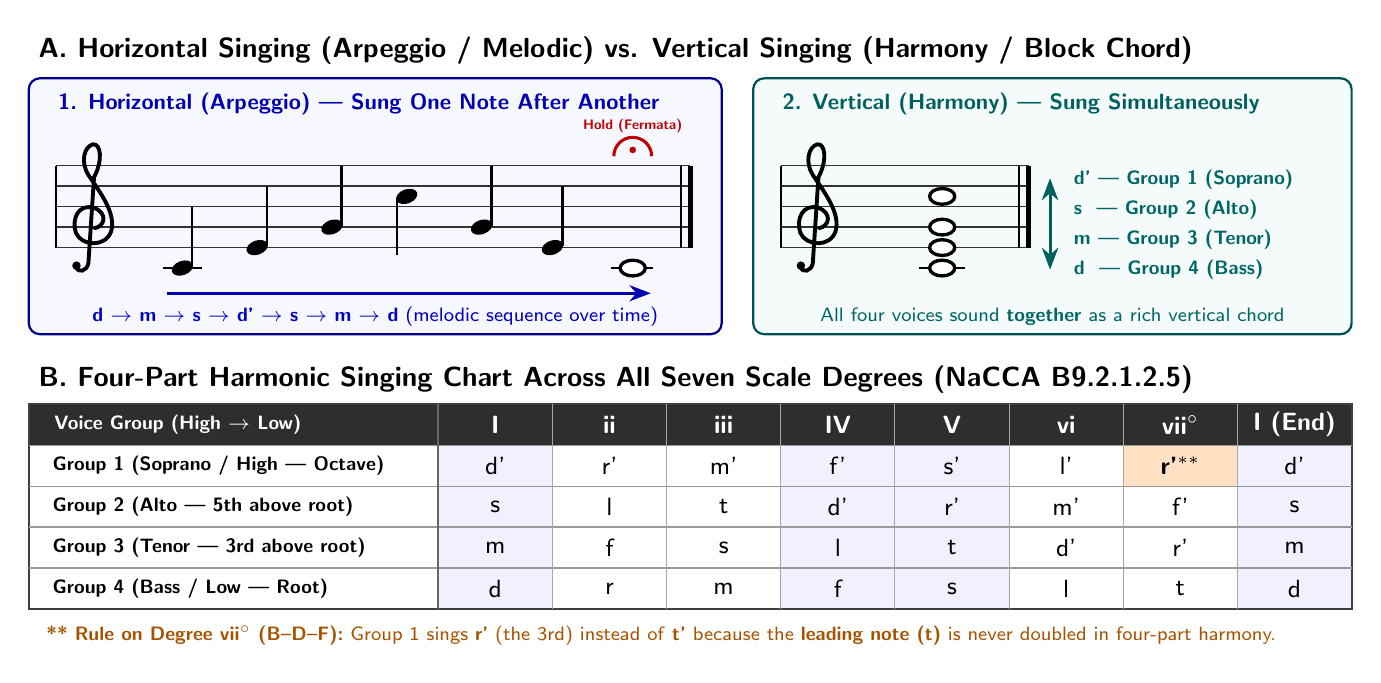
\begin{tikzpicture}[
    font=\sffamily,
    >=Stealth
]

\newcommand{\crotchetup}[2]{%
    \fill[black, rotate around={20:(#1,#2)}] (#1,#2) ellipse (0.14 and 0.09);
    \draw[line width=0.95pt] (#1+0.125, #2+0.02) -- (#1+0.125, #2+0.78);
}
\newcommand{\wholenote}[2]{%
    \fill[white] (#1, #2) ellipse (0.16 and 0.10);
    \draw[line width=1.2pt, black] (#1, #2) ellipse (0.16 and 0.10);
}

% ================= TOP PANEL: HORIZONTAL vs VERTICAL =================
\node[font=\sffamily\bfseries\normalsize, anchor=west] at (0, 7.65)
    {A. Horizontal Singing (Arpeggio / Melodic) vs. Vertical Singing (Harmony / Block Chord)};

% Left Box: Horizontal Arpeggio (x = 0 .. 8.8, y = 4.05 .. 7.30)
\draw[rounded corners=4pt, draw=blue!55!black, fill=blue!3, line width=0.8pt] (0, 4.05) rectangle (8.8, 7.30);
\node[font=\sffamily\bfseries\footnotesize, text=blue!70!black, anchor=west] at (0.25, 6.98)
    {1. Horizontal (Arpeggio) --- Sung One Note After Another};

% Staff inside Left Box (y base = 5.15, spacing 0.26)
\begin{scope}[shift={(0.35, 5.15)}]
    \foreach \k in {0,1,2,3,4} {
        \draw[line width=0.55pt, black!80] (0, \k*0.26) -- (8.05, \k*0.26);
    }
    \draw[line width=0.8pt] (0, 0) -- (0, 1.04);
    \draw[line width=0.7pt] (7.93, 0) -- (7.93, 1.04);
    \draw[line width=1.8pt] (8.05, 0) -- (8.05, 1.04);

    % Treble clef
    \begin{scope}[shift={(0.45, 0.26)}, scale=0.72]
        \draw[line width=1.4pt, black, line cap=round]
            (0.05, -0.02)
            .. controls (0.24, 0.02) and (0.28, 0.25) .. (0.04, 0.34)
            .. controls (-0.24, 0.42) and (-0.36, 0.14) .. (-0.28, -0.10)
            .. controls (-0.18, -0.34) and (0.24, -0.36) .. (0.34, -0.08)
            .. controls (0.44, 0.24) and (0.14, 0.62) .. (-0.06, 0.92)
            .. controls (-0.20, 1.14) and (-0.14, 1.42) .. (0.02, 1.46)
            .. controls (0.16, 1.48) and (0.20, 1.18) .. (0.04, 0.88)
            -- (-0.06, -0.64)
            .. controls (-0.09, -0.78) and (-0.24, -0.82) .. (-0.28, -0.70);
        \fill[black] (-0.27, -0.68) circle (0.075);
    \end{scope}

    % Arpeggio notes: C4 (-0.26), E4 (0), G4 (0.26), C5 (0.65), G4, E4, C4 (held with fermata)
    \draw[line width=0.65pt] (1.35, -0.26) -- (1.85, -0.26);
    \crotchetup{1.60}{-0.26}
    \crotchetup{2.55}{0.00}
    \crotchetup{3.50}{0.26}
    % C5 stem down
    \fill[black, rotate around={20:(4.45,0.65)}] (4.45,0.65) ellipse (0.14 and 0.09);
    \draw[line width=0.95pt] (4.45-0.125, 0.65-0.02) -- (4.45-0.125, 0.65-0.75);
    \crotchetup{5.40}{0.26}
    \crotchetup{6.30}{0.00}
    % Final held C4 (whole note + fermata)
    \draw[line width=0.65pt] (7.05, -0.26) -- (7.58, -0.26);
    \wholenote{7.32}{-0.26}
    % Fermata sign cleanly placed above staff with space below box title
    \draw[line width=1.1pt, red!75!black] (7.08, 1.16) arc[start angle=180, end angle=0, radius=0.24];
    \fill[red!75!black] (7.32, 1.24) circle (0.042);
    \node[font=\sffamily\tiny\bfseries, text=red!75!black] at (7.32, 1.54) {Hold (Fermata)};

    % Time-flow arrow + caption cleanly separated
    \draw[->, line width=1.05pt, blue!70!black] (1.40, -0.58) -- (7.55, -0.58);
    \node[font=\sffamily\scriptsize, text=blue!75!black] at (4.05, -0.88)
        {\textbf{d $\to$ m $\to$ s $\to$ d' $\to$ s $\to$ m $\to$ d} (melodic sequence over time)};
\end{scope}

% Right Box: Vertical Harmony (x = 9.2 .. 16.8, y = 4.05 .. 7.30)
\draw[rounded corners=4pt, draw=teal!65!black, fill=teal!4, line width=0.8pt] (9.2, 4.05) rectangle (16.8, 7.30);
\node[font=\sffamily\bfseries\footnotesize, text=teal!75!black, anchor=west] at (9.45, 6.98)
    {2. Vertical (Harmony) --- Sung Simultaneously};

\begin{scope}[shift={(9.55, 5.15)}]
    % Compact staff on left half of right box (0 .. 3.10) so voice labels sit in clean white space!
    \foreach \k in {0,1,2,3,4} {
        \draw[line width=0.55pt, black!80] (0, \k*0.26) -- (3.15, \k*0.26);
    }
    \draw[line width=0.8pt] (0, 0) -- (0, 1.04);
    \draw[line width=0.7pt] (3.03, 0) -- (3.03, 1.04);
    \draw[line width=1.8pt] (3.15, 0) -- (3.15, 1.04);

    % Treble clef
    \begin{scope}[shift={(0.45, 0.26)}, scale=0.72]
        \draw[line width=1.4pt, black, line cap=round]
            (0.05, -0.02)
            .. controls (0.24, 0.02) and (0.28, 0.25) .. (0.04, 0.34)
            .. controls (-0.24, 0.42) and (-0.36, 0.14) .. (-0.28, -0.10)
            .. controls (-0.18, -0.34) and (0.24, -0.36) .. (0.34, -0.08)
            .. controls (0.44, 0.24) and (0.14, 0.62) .. (-0.06, 0.92)
            .. controls (-0.20, 1.14) and (-0.14, 1.42) .. (0.02, 1.46)
            .. controls (0.16, 1.48) and (0.20, 1.18) .. (0.04, 0.88)
            -- (-0.06, -0.64)
            .. controls (-0.09, -0.78) and (-0.24, -0.82) .. (-0.28, -0.70);
        \fill[black] (-0.27, -0.68) circle (0.075);
    \end{scope}

    % Stacked C-E-G-C' chord at x = 2.05
    \draw[line width=0.65pt] (1.76, -0.26) -- (2.34, -0.26);
    \wholenote{2.05}{-0.26}
    \wholenote{2.05}{0.00}
    \wholenote{2.05}{0.26}
    \wholenote{2.05}{0.65}

    % Clean vertical alignment arrow & voice labels OUTSIDE the staff to the right!
    \draw[<->, line width=1.1pt, teal!75!black] (3.42, -0.28) -- (3.42, 0.88);
    \node[font=\sffamily\scriptsize\bfseries, text=teal!80!black, anchor=west] at (3.60, 0.86) {d' --- Group 1 (Soprano)};
    \node[font=\sffamily\scriptsize\bfseries, text=teal!80!black, anchor=west] at (3.60, 0.48) {s \ --- Group 2 (Alto)};
    \node[font=\sffamily\scriptsize\bfseries, text=teal!80!black, anchor=west] at (3.60, 0.10) {m --- Group 3 (Tenor)};
    \node[font=\sffamily\scriptsize\bfseries, text=teal!80!black, anchor=west] at (3.60, -0.28) {d \ --- Group 4 (Bass)};

    \node[font=\sffamily\scriptsize, text=teal!80!black] at (3.45, -0.88)
        {All four voices sound \textbf{together} as a rich vertical chord};
\end{scope}

% ================= BOTTOM PANEL: 4-PART CHORAL VOICE CHART =================
\node[font=\sffamily\bfseries\normalsize, anchor=west] at (0, 3.48)
    {B. Four-Part Harmonic Singing Chart Across All Seven Scale Degrees (NaCCA B9.2.1.2.5)};

% Table geometry: total width = 16.8; Col 0 = 0..5.20; 8 degree cols of width 1.45 each (5.20 + 8*1.45 = 16.80)
\def\ytop{3.16}
\def\rh{0.52}

% Header row
\fill[black!82] (0, \ytop-\rh) rectangle (16.8, \ytop);
\node[font=\sffamily\bfseries\scriptsize, text=white, anchor=west] at (0.20, \ytop-0.26) {Voice Group (High $\to$ Low)};
\foreach \i/\lbl in {0/I, 1/ii, 2/iii, 3/IV, 4/V, 5/vi, 6/{vii$^\circ$}, 7/{I (End)}} {
    \pgfmathsetmacro{\xc}{5.20 + \i*1.45 + 0.725}
    \node[font=\sffamily\bfseries\small, text=white] at (\xc, \ytop-0.26) {\lbl};
}

% Highlight primary columns I, IV, V, I(End) and special cell (Group 1, vii°)
\foreach \col in {0,3,4,7} {
    \pgfmathsetmacro{\xl}{5.20 + \col*1.45}
    \fill[blue!6] (\xl, \ytop-5*\rh) rectangle (\xl+1.45, \ytop-\rh);
}
\fill[orange!24] (5.20+6*1.45, \ytop-2*\rh) rectangle (5.20+7*1.45, \ytop-\rh);

% Row labels
\foreach \r/\vname in {
    1/{Group 1 (Soprano / High --- Octave)},
    2/{Group 2 (Alto --- 5th above root)},
    3/{Group 3 (Tenor --- 3rd above root)},
    4/{Group 4 (Bass / Low --- Root)}
} {
    \pgfmathsetmacro{\yc}{\ytop - \r*\rh - 0.26}
    \node[font=\sffamily\bfseries\scriptsize, anchor=west] at (0.18, \yc) {\vname};
}

% Group 1..4 solfa cells
\foreach \i/\val in {0/d', 1/r', 2/m', 3/f', 4/s', 5/l', 6/{\textbf{r'$^{**}$}}, 7/d'} {
    \pgfmathsetmacro{\xc}{5.20 + \i*1.45 + 0.725}
    \node[font=\sffamily\small] at (\xc, \ytop-1*\rh-0.26) {\val};
}
\foreach \i/\val in {0/s, 1/l, 2/t, 3/d', 4/r', 5/m', 6/f', 7/s} {
    \pgfmathsetmacro{\xc}{5.20 + \i*1.45 + 0.725}
    \node[font=\sffamily\small] at (\xc, \ytop-2*\rh-0.26) {\val};
}
\foreach \i/\val in {0/m, 1/f, 2/s, 3/l, 4/t, 5/d', 6/r', 7/m} {
    \pgfmathsetmacro{\xc}{5.20 + \i*1.45 + 0.725}
    \node[font=\sffamily\small] at (\xc, \ytop-3*\rh-0.26) {\val};
}
\foreach \i/\val in {0/d, 1/r, 2/m, 3/f, 4/s, 5/l, 6/t, 7/d} {
    \pgfmathsetmacro{\xc}{5.20 + \i*1.45 + 0.725}
    \node[font=\sffamily\small] at (\xc, \ytop-4*\rh-0.26) {\val};
}

% Grid borders
\draw[line width=0.75pt, black!75] (0, \ytop-5*\rh) rectangle (16.8, \ytop);
\foreach \r in {1,2,3,4} {
    \draw[line width=0.45pt, black!40] (0, \ytop-\r*\rh) -- (16.8, \ytop-\r*\rh);
}
\draw[line width=0.6pt, black!60] (5.20, \ytop-5*\rh) -- (5.20, \ytop);
\foreach \i in {1,...,7} {
    \pgfmathsetmacro{\xl}{5.20 + \i*1.45}
    \draw[line width=0.4pt, black!35] (\xl, \ytop-5*\rh) -- (\xl, \ytop);
}

% Footnote
\node[font=\sffamily\scriptsize, anchor=west, text=orange!65!black] at (0.10, 0.22)
    {\textbf{** Rule on Degree vii$^\circ$ (B--D--F):} Group 1 sings \textbf{r'} (the 3rd) instead of \textbf{t'} because the \textbf{leading note (t)} is never doubled in four-part harmony.};

\end{tikzpicture}
\end{document}
